\documentclass{harvardml}

\course{CS281-F17}
\assignment{CS281 Section \#6 Notes, v 1.1 NZ}

\usepackage{url, enumitem}
\usepackage{amsfonts, amsmath, amsthm}
\usepackage{listings}
\usepackage{hyperref}

\theoremstyle{definition}
\newtheorem{defn}{Definition}[section]
\theoremstyle{plain}
\usepackage[textsize=tiny]{todonotes}

% Some useful macros.
\newcommand{\given}{\,|\,}
\newcommand{\R}{\mathbb{R}}
\newcommand{\C}{\mathbb{C}}
\newcommand{\E}{\mathbb{E}}
\newcommand{\var}{\text{var}}
\newcommand{\cov}{\text{cov}}
\newcommand{\p}{\partial}
\newcommand{\mba}{\mathbf{a}}
\newcommand{\mbb}{\mathbf{b}}
\newcommand{\mbx}{\mathbf{x}}
\newcommand{\mcX}{\mathcal{X}}
\newcommand{\mcY}{\mathcal{Y}}
\newcommand{\boldw}{\mathbf{w}}
\newcommand{\mbxt}{\tilde{\mathbf{x}}}
\newcommand{\Sigmat}{\tilde{\Sigma}}
\newcommand{\mbz}{\mathbf{z}}
\newcommand{\mbw}{\mathbf{w}}
\newcommand{\mcN}{\mathcal{N}}
\newcommand{\mcP}{\mathcal{P}}
\newcommand{\eps}{\epsilon}
\newcommand{\trans}{\intercal}
\newcommand{\Ut}{\tilde{U}}
\DeclareMathOperator*{\argmax}{arg\,max}
\newcommand{\angstrom}{\textup{\AA}}
\renewcommand{\v}[1]{\mathbf{#1}}
\newcommand{\on}{\operatorname}

\newtheorem{theorem}{Theorem}
\newtheorem*{proposition}{Proposition}
\newtheorem{lemma}[theorem]{Lemma}
\newtheorem{corollary}[theorem]{Corollary}
\newtheorem{conjecture}[theorem]{Conjecture}
\newtheorem{postulate}[theorem]{Postulate}
\theoremstyle{definition}
\newtheorem{example}[theorem]{Example}

\theoremstyle{remark}
\newtheorem*{remark}{Remark}
\newtheorem*{notation}{Notation}
\newtheorem*{note}{Note}

\hypersetup{
    colorlinks=true,
    linkcolor=blue,
    filecolor=magenta,      
    urlcolor=blue,
}

%%%%%% for the dags %%%%%%%
\usetikzlibrary{arrows}
\tikzset{
    vertex/.style={circle,draw,minimum size=1.5em},
    dedge/.style={->,> = latex'},
    edge/.style={-,> = latex', draw=black},
    msgup/.style={->,> = latex', draw=magenta},
    msgdown/.style={->,> = latex', draw=cyan},
    msg/.style={->,> = latex', draw=green},
    given/.style={circle,draw,minimum size=1.5em, fill=gray},
}


%%%%%%%%%%%%%%%%%%%%%%%%%%%%%

\begin{document}


\section{Distributive Property}
\subsection{Review and Walkthrough}
We are interested in calculating the marginal probability of a random variable $x_i$ in our graphical model. However, we have so many other variables that summing over all of these other variables in the joint distribution can quickly be infeasible. We will use a key idea, "\emph{pushing sums inside products}", which is just to say that multiplication distributes over addition:
$$\sum_i\sum_j\sum_k a_i b_j c_k =\sum_i a_i\left[\sum_j b_j \left(\sum_k c_k\right)\right]$$
but for $i\in [0,1], j \in [0,1,2], k \in [0,1,2,3]$ the LHS corresponds to 48 multiplications and 23 additions whereas the RHS is only 5 multiplications and 6 additions!

\medskip 
We will walk through applying the distributive property on the following UGM:

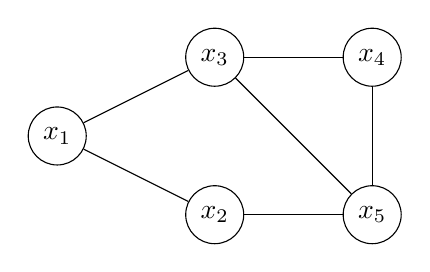
\begin{tikzpicture}
\node[vertex] (1) at (0,0) {$x_1$};
\node[vertex] (2) at (2,-1) {$x_2$};
\node[vertex] (3) at (2,1) {$x_3$}; \node[vertex] (4) at (4,1) {$x_4$};
\node[vertex] (5) at (4,-1) {$x_5$};
\draw[edge] (1) --(3);
\draw[edge] (3) --(5);
\draw[edge] (3) --(4);
\draw[edge] (4) --(5);
\draw[edge] (2) --(5);
\draw[edge] (1)--(2);
\end{tikzpicture}

We factor the joint probability distribution for our UGM by the potential functions for maximal cliques:
$$p(\mathbf{X}) \propto \psi_{12}(x_1, x_2)
\psi_{13}(x_1, x_3)
\psi_{25}(x_2, x_5)
\psi_{345}(x_3, x_4, x_5)$$

Suppose we are interested in the marginal probability of $x_1$. We have that:

\begin{align*}
p(x_1) &= \sum_{x_2 : x_5} p(\mathbf{X})\\
&= \sum_{x_2 : x_5} \psi_{12}(x_1, x_2)
\psi_{13}(x_1, x_3)
\psi_{25}(x_2, x_5)
\psi_{345}(x_3, x_4, x_5)
\end{align*}

From here, we can see that the order in which we sum out variables can make a difference. Consider the elimination ordering $(x_5, x_4, x_3, x_2)$:

\begin{align*}
p(x_1) &= \sum_{x_2 : x_5} \psi_{12}(x_1, x_2)
\psi_{13}(x_1, x_3)
\psi_{25}(x_2, x_5)
\psi_{345}(x_3, x_4, x_5)\\
&= \sum_{x_2: x_4} \psi_{12}(x_1, x_2)
\psi_{13}(x_1, x_3)
\underbrace{
\sum_{x_5}
\psi_{25}(x_2, x_5)
\psi_{345}(x_3, x_4, x_5)}_\text{$m_5(2,3,4)$}\\
\end{align*}

(The notation here foreshadows that $m_5(2,3,4) = \sum_{x_5}\psi_{25}(x_2, x_5)
\psi_{345}(x_3, x_4, x_5)$ can be thought of as the 'message' from 5 to its neighbors 2, 3, and 4.) 

Continuing on in this way, we have:

\begin{align*}
p(x_1) &= \sum_{x_2:x_4} \psi_{12}(x_1, x_2)
\psi_{13}(x_1, x_3)
m_5(2,3,4)\\
&= \sum_{x_2:x_3}\psi_{12}(x_1, x_2)
\psi_{13}(x_1, x_3)
\underbrace{\sum_{x_4}m_5(2,3,4)}_\text{$m_4(x_2, x_3)$}\\
&= \sum_{x_2: x_3}\psi_{12}(x_1, x_2)
\psi_{13}(x_1, x_3)m_4(x_2, x_3)\\
&= \sum_{x_2} \psi_{12}(x_1, x_2) \underbrace{\sum_{x_3} \psi_{13}(x_1, x_3)m_4(x_2, x_3)}_\text{$m_3(x_1, x_2)$}\\
&= \sum_{x_2} \psi_{12}(x_1, x_2)m_3(x_1, x_2) = m_2(x_1)
\end{align*}

Then we just need to normalize $m_2(x_1)$ to calculate the marginal probability on $x_1$.

% take out questions 
% \begin{itemize}
%     \item What was the most expensive summation? What would have been a more efficient elimination ordering?
%     \item What if we had observed $x_2$?
% \end{itemize}

\section{Belief Propagation for Trees}
\subsection{Motivation, Review}
\begin{itemize}
    \item  For an undirected tree, the edges are exactly the maximal cliques
    \item The Hammersley-Clifford Theorem: represent the joint distribution as the product of potentials $\psi_{i,j}(i,j)$ for each edge.
    \item Murphy and class notation includes unary potentials. So we have a tree represented by 
    
    $$p(\mathbf{x}|\mathbf{v}) = \frac{1}{Z(v)} \prod_{s \in \nu} \psi_s(x_s) \prod_{(s,t) \in E} \psi_{(s,t)}(x_s,x_t)$$
\end{itemize}

Consider the following tree
\begin{center}
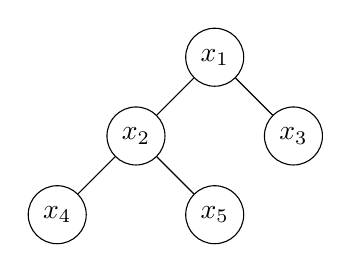
\begin{tikzpicture}
\node[vertex] (1) at (0,0) {$x_1$};
\node[vertex] (2) at (-1, -1) {$x_2$};
\node[vertex] (3) at (1, -1) {$x_3$};
\node[vertex] (4) at (-2, -2) {$x_4$};
\node[vertex] (5) at (0, -2) {$x_5$};
\draw[edge] (1) --(2);
\draw[edge] (1) --(3);
\draw[edge] (2) --(4);
\draw[edge] (2) --(5);
\end{tikzpicture}
\end{center}

Suppose we want to compute the marginal for $x_3$. Pushing sums inside products with an ordering of $(5,4,2,1)$, we would have to calculate and store the following messages:
\begin{center}
\begin{align*}
    m_5(x_2) &= \sum_{x_5} \psi_5(x_5) \psi_{2,5}(x_2, x_5)\\
    m_4(x_2) &= \sum_{x_4}\psi_4(x_4) \psi_{2,4}(x_2, x_4)\\
    m_2(x_1) &= \sum_{x_2}\psi_2(x_2) \psi_{1,2}(x_1, x_2) m_4(x_2) m_5(x_2)\\
    m_1(x_3) &= \sum_{x_1} \psi_1(x_1) \psi_{1,3}(x_1, x_3) m_2(x_1) m_4(x_2) m_5(x_2)
\end{align*}
\end{center}

% % TODO: label edges with messages 
% \begin{center}
% \begin{tikzpicture}
% \node[vertex] (1) at (0,0) {$x_1$};
% \node[vertex] (2) at (-1, -1) {$x_2$};
% \node[vertex] (3) at (1, -1) {$x_3$};
% \node[vertex] (4) at (-2, -2) {$x_4$};
% \node[vertex] (5) at (0, -2) {$x_5$};
% \draw[dedge] (5) --(2);
% \draw[dedge] (4) --(2);
% \draw[dedge] (2) --(1);
% \draw[dedge] (1) --(3);
% \end{tikzpicture}
% \end{center}
% [TODO maybe this graph is confusing because the edges are not what we usually think of as 'edges' but just show the directionality of the messages.]

Similarly, to compute the marginal for $x_1$ with  elimination ordering $(4,5,3,2,1)$, the following messages would be needed:

\begin{center}
\begin{align*}
    m_4(x_2) &= \sum_{x_4} \psi(x_4)\psi(x_4, x_2)\\
    m_5(x_2) &= \sum_{x_5} \psi(x_5)\psi(x_5, x_2)\\
    m_3(x_1) &= \sum_{x_3} \psi(x_3) \psi(x_3, x_1)\\
    m_2(x_1) &= \sum_{x_2} \psi(x_2) \psi(x_2, x_1) m_5(x_2) m_4(x_2)
\end{align*}
\end{center}

So that
\begin{center}
\begin{align*}
p(x_1) &\propto \sum_{x_2:x_5} \psi_1(x_1) \psi_2(x_2) \psi_3(x_3) \psi_4(x_4) \psi_5(x_5) \psi(x_1,x_3) \psi(x_1,x_2) \psi(x_2,x_4) \psi(x_2,x_5)\\
&=\psi_1(x_1) m_3(x_1) m_2(x_1)\\
\end{align*}
\end{center}

Notice the following:
\begin{itemize}
\item We see that to compute the marginal probability at node $x_1$, we multiply its unary potential with all its incoming messages:

$$p(x_i)\propto \psi_i(x_i)\prod_{n \in \text{neighbors}(i)}m_{n \rightarrow i}(x_i)$$

In this case, it is the messages from $x_3$ and $x_2$. However, these messages that $x_3$ and $x_2$ deliver to $x_1$ also depends on messages from \emph{their} neighbors. More formally, to compute the message $m_{s \rightarrow t}(x_t)$, we need to have already computed the messages from the incoming neighbors of s: $m_{r \rightarrow s}(x_s)$ for $r \in N(s) \setminus t$. 
\item In computing the marginals for $x_1$ and $x_3$, we need some of the same computations, namely, 
$m_4(x_2), m_5(x_2), \\m_2(x_1)$. 
It would be nice to have a procedure that identifies and caches these computations that are `reused' for the calculations of all marginal probabilities of interest.   
\end{itemize}


This can be done through \emph{belief propagation}, also called \emph{sum-product algorithm on trees}. We can think of the partial sums reused to calculate marginals as the \emph{messages}. Belief propagation also has a nice effect that we will end up calculating all the marginals (\emph{beliefs}) for our tree.\\

\subsection{Sequential Belief Propagation}
The sequential implementation of belief propagation is as follows:  
\begin{itemize}
    \item Pick an arbitrary node as the root. This will give the tree an ordering of parent, child relationships.
    For example, if we pick $x_2$ to be the root, we can represent the parent-child relationships with the following graph, where the directed edge indicates $\text{parent} \rightarrow \text{child}$. Note our tree itself is still an undirected tree - the directed edges only have meaning relative to the chosen root. 
    
    \begin{center}
    
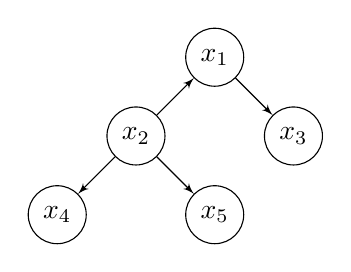
\begin{tikzpicture}
\node[vertex] (1) at (0,0) {$x_1$};
\node[vertex] (2) at (-1, -1) {$x_2$};
\node[vertex] (3) at (1, -1) {$x_3$};
\node[vertex] (4) at (-2, -2) {$x_4$};
\node[vertex] (5) at (0, -2) {$x_5$};
\draw[dedge] (2) --(4);
\draw[dedge] (2) --(5);
\draw[dedge] (2) --(1);
\draw[dedge] (1) --(3);
\end{tikzpicture}
\end{center}

    
    \item Bottom up (leaves to root): 
    Graphically, we calculate these messages:\\
    (Note) Each graph below shows multiple time steps. In the serial BP procedure, a node can only send a message after it has received all its messages, so we proceed one by one starting with a leaf node. 
    
\begin{center}
    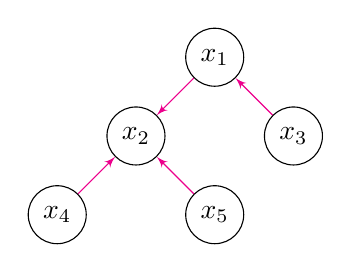
\begin{tikzpicture}
    \node[vertex] (1) at (0,0) {$x_1$};
    \node[vertex] (2) at (-1, -1) {$x_2$};
    \node[vertex] (3) at (1, -1) {$x_3$};
    \node[vertex] (4) at (-2, -2) {$x_4$};
    \node[vertex] (5) at (0, -2) {$x_5$};
    \draw[msgup] (5) --(2);
    \draw[msgup] (4) --(2);
    \draw[msgup] (3) --(1);
    \draw[msgup] (1) --(2);
    \end{tikzpicture}
\end{center}

Defns (Murphy):
\begin{align*}m_{s\rightarrow t}^{-}(x_t) &= \sum_{x_s}\psi_{s,t}(x_s, x_t)\text{bel}_s^{-}(x_s)\\
\text{bel}_s^{-}(x_s) &= \frac{1}{Z_s}\psi_s(x_s)\prod_{c \in \text{Ch}(s)}m_{c\rightarrow s}^{-}(x_s)
\end{align*}

So on the bottom up sweep of belief propagation, we have calculated:
    \begin{align*}
        m_{4 \rightarrow 2}^{-}(x_2) &= \sum_{x_4} \psi_{2,4}(x_2,x_4) \text{bel}_4^{-}(x_4) = \sum_{x_4} \psi_{2,4}(x_2,x_4)\psi_4(x_4)\\ % since leaf node\\
        m_{5 \rightarrow 2}^{-}(x_2) &= \sum_{x_5} \psi_{2,5}(x_2,x_5) \psi_5(x_5)\\
        \\
        m_{3 \rightarrow 1}^{-}(x_1) &= \sum_{x_3} \psi_{1,3}(x_1, x_3) \psi_3(x_3)\\
        m_{1 \rightarrow 2}^{-}(x_2) &= \sum_{x_1} \psi_{1,2}(x_1, x_2) \text{bel}_1^{-}(x_1)\\
        &= \sum_{x_1} \psi_{1,2}(x_1, x_2) \psi_1(x_1)m_{3 \rightarrow 1}(x_1)
    \end{align*}
In the upward sweep, we have calculated half of the $2(N-1)$ total messages in our graph. 
    
    
    \item Top down (root to leaves):\\
     We will be calculating these top-down messages:
    
\begin{center}
    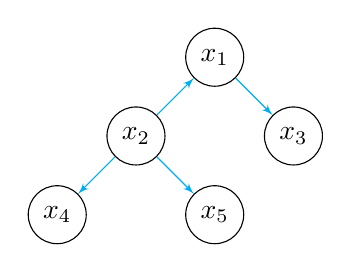
\begin{tikzpicture}
    \node[vertex] (1) at (0,0) {$x_1$};
    \node[vertex] (2) at (-1, -1) {$x_2$};
    \node[vertex] (3) at (1, -1) {$x_3$};
    \node[vertex] (4) at (-2, -2) {$x_4$};
    \node[vertex] (5) at (0, -2) {$x_5$};
    \draw[msgdown] (2) --(5);
    \draw[msgdown] (2) --(4);
    \draw[msgdown] (2) --(1);
    \draw[msgdown] (1) --(3);
    \end{tikzpicture}
\end{center}

Since a node can only send an outgoing message if it has received all of its incoming messages, we see that we will reuse our previous bottom-up messages in our calculations for top-down messages. For example, the outgoing top-down message from $x_2$ to $x_4$ relies on the incoming messages to $x_2$. By design, we have already calculated these!

\begin{center}
    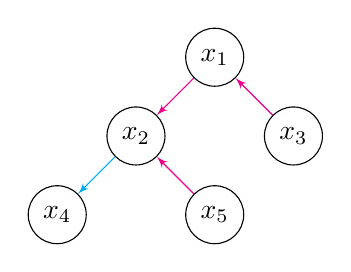
\begin{tikzpicture}
    \node[vertex] (1) at (0,0) {$x_1$};
    \node[vertex] (2) at (-1, -1) {$x_2$};
    \node[vertex] (3) at (1, -1) {$x_3$};
    \node[vertex] (4) at (-2, -2) {$x_4$};
    \node[vertex] (5) at (0, -2) {$x_5$};
    \draw[msgup] (5) --(2);
    \draw[msgdown] (2) --(4);
    \draw[msgup] (1) --(2);
    \draw[msgup] (3) --(1);
    \end{tikzpicture}
\end{center}

Formally:
$$m_{t \rightarrow s}^{+} (x_s) = \sum_{x_t}\psi_{s,t}(x_s,x_t)\psi_t(x_t) 
\textcolor{magenta}{\prod_{c \in \text{ch}(t)\setminus s} m_{c \rightarrow t}^{-}(x_t)} \textcolor{cyan}{\prod_{p \in pa(t)} m_{p \rightarrow t}^{+}(x_t)}$$

So the messages we produce on the top-down sweep are:

\begin{align*}
    m_{2 \rightarrow 4}^{+} (x_4) &= \sum_{x_2} \psi_{2,4}(x_2,x_4)\psi_2(x_2) \textcolor{magenta}{m_{5 \rightarrow 2}^{-}(x_2)  m_{1 \rightarrow 2}^{-}(x_2)}\\ %x2 has no parents
    m_{2 \rightarrow 5}^{+} (x_5) &= \sum_{x_2} \psi_{2,5}(x_2,x_5)\psi_2(x_2) \textcolor{magenta}{m_{4 \rightarrow 2}^{-}(x_2)  m_{1 \rightarrow 2}^{-}(x_2)}\\
    m_{2 \rightarrow 1}^{+} (x_1) &= \sum_{x_2} \psi_{2,1}(x_2,x_1)\psi_2(x_2) \textcolor{magenta}{m_{4 \rightarrow 2}^{-}(x_2)  m_{5 \rightarrow 2}^{-}(x_2)}\\
    m_{1 \rightarrow 3}^{+} (x_3) &= \sum_{x_1} \psi_{1,3}(x_1,x_3)\psi_2(x_2) \textcolor{cyan}{m_{2 \rightarrow 1}^{+}(x_1)}\\
\end{align*}
\end{itemize}
\medskip 

In doing both the bottom-up and top-down sweeps, we have calculated \emph{all} the messages needed to find the beliefs at \emph{every node}. This is perhaps best shown graphically: 
\begin{itemize}
\item After doing the steps above, calculating belief at node $x_1$ requires:\\
$\text{bel}(x_1) \propto \psi_1(x_1)m_{2 \rightarrow 1}^{+}(x_1)m_{3 \rightarrow 1}^{-}(x_1)$, and indeed we have the required messages to compute $m_{2 \rightarrow 1}^{+}(x_1)$
\begin{center}
    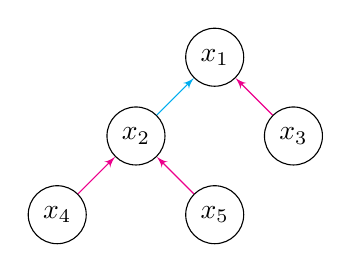
\begin{tikzpicture}
    \node[vertex] (1) at (0,0) {$x_1$};
    \node[vertex] (2) at (-1, -1) {$x_2$};
    \node[vertex] (3) at (1, -1) {$x_3$};
    \node[vertex] (4) at (-2, -2) {$x_4$};
    \node[vertex] (5) at (0, -2) {$x_5$};
    \draw[msgup] (3) --(1);
    \draw[msgup] (4) --(2);
    \draw[msgup] (5) --(2);
    \draw[msgdown] (2) --(1);
    \end{tikzpicture}
\end{center}



\item Calculating the belief at node $x_3$ requires the following messages: $\text{bel}(x_3) \propto \psi_3(x_3)m_{1 \rightarrow 3}^{+}(x_3)$
\begin{center}
    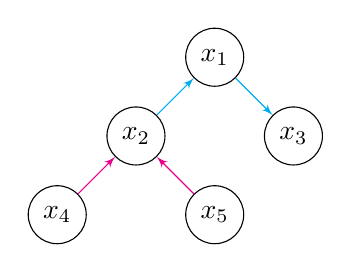
\begin{tikzpicture}
    \node[vertex] (1) at (0,0) {$x_1$};
    \node[vertex] (2) at (-1, -1) {$x_2$};
    \node[vertex] (3) at (1, -1) {$x_3$};
    \node[vertex] (4) at (-2, -2) {$x_4$};
    \node[vertex] (5) at (0, -2) {$x_5$};
    \draw[msgdown] (1) --(3);
    \draw[msgup] (4) --(2);
    \draw[msgup] (5) --(2);
    \draw[msgdown] (2) --(1);
    \end{tikzpicture}
\end{center}

\item We get the belief for node $x_2$ just from the upward pass, since we chose $x_2$ to be our root node: $\text{bel}(x_2) \propto \psi_2(x_2)m_{1 \rightarrow 2}^{-}(x_2)m_{4 \rightarrow 2}^{-}(x_2)m_{5 \rightarrow 2}^{-}(x_2)$
\begin{center}
    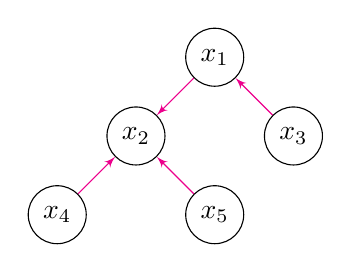
\begin{tikzpicture}
    \node[vertex] (1) at (0,0) {$x_1$};
    \node[vertex] (2) at (-1, -1) {$x_2$};
    \node[vertex] (3) at (1, -1) {$x_3$};
    \node[vertex] (4) at (-2, -2) {$x_4$};
    \node[vertex] (5) at (0, -2) {$x_5$};
    \draw[msgup] (3) --(1);
    \draw[msgup] (4) --(2);
    \draw[msgup] (5) --(2);
    \draw[msgup] (1) --(2);
    \end{tikzpicture}
\end{center}
\end{itemize}


\subsection{Parallel Belief Propagation}
The BP algorithm in the previous section is inherently sequential. But we can also implement BP in parallel. We no longer pick a root node and propagate messages up and down. Instead, at every time step, we propagate outgoing messages from all nodes that are ready to send them, i.e. all nodes that have received all their other incoming messages.\\
\medskip

    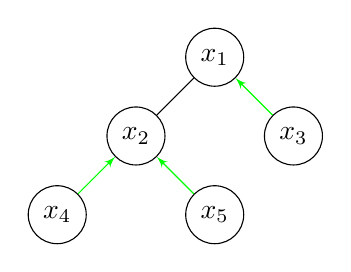
\begin{tikzpicture}
    \node[vertex] (1) at (0,0) {$x_1$};
    \node[vertex] (2) at (-1, -1) {$x_2$};
    \node[vertex] (3) at (1, -1) {$x_3$};
    \node[vertex] (4) at (-2, -2) {$x_4$};
    \node[vertex] (5) at (0, -2) {$x_5$};
    \draw[msg] (3) --(1);
    \draw[msg] (4) --(2);
    \draw[msg] (5) --(2);
    \draw[edge] (1) --(2);
    \end{tikzpicture}
    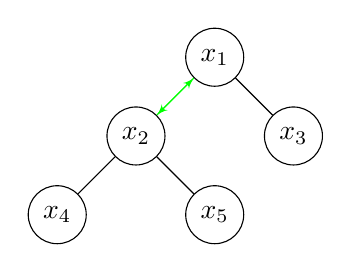
\begin{tikzpicture}
    \node[vertex] (1) at (0,0) {$x_1$};
    \node[vertex] (2) at (-1, -1) {$x_2$};
    \node[vertex] (3) at (1, -1) {$x_3$};
    \node[vertex] (4) at (-2, -2) {$x_4$};
    \node[vertex] (5) at (0, -2) {$x_5$};
    \draw[edge] (3) --(1);
    \draw[edge] (4) --(2);
    \draw[edge] (5) --(2);
    \draw[msg] (1) --(2);
    \draw[msg] (2) --(1);
    \end{tikzpicture}
    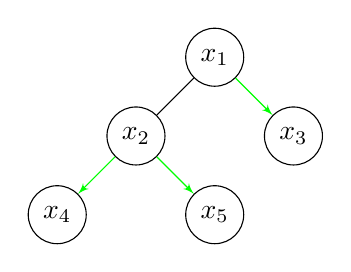
\begin{tikzpicture}
    \node[vertex] (1) at (0,0) {$x_1$};
    \node[vertex] (2) at (-1, -1) {$x_2$};
    \node[vertex] (3) at (1, -1) {$x_3$};
    \node[vertex] (4) at (-2, -2) {$x_4$};
    \node[vertex] (5) at (0, -2) {$x_5$};
    \draw[msg] (1) --(3);
    \draw[msg] (2) --(4);
    \draw[msg] (2) --(5);
    \draw[edge] (2) --(1);
    \end{tikzpicture}
\medskip 

\noindent After these 3 time steps, we have computed all the messages needed to find beliefs at every node. The procedure is equivalent to serial BP.

The serial Belief Propagation is optimal for tree structure. For a graph with loop, we could still use parallel BP to get approximation marginals. At each step, all nodes receive messages from their neighbors in parallel, update their belief states, $$\text{bel}_s (x_s) \propto\psi_s(x_s)\prod_{c \in \text{nb}(s)}m_{c\rightarrow s}(x_s)$$
and finally send new messages back out to their neighbors: $$m_{s \rightarrow t} (x_t) = \sum_{x_s}\psi_{s,t}(x_s,x_t)\psi_s(x_s)\prod_{c \in \text{nb}(s)\setminus t} m_{c \rightarrow s}(x_s) $$
This process repeats until convergence. 


\subsection{Only Trees Please}
BP can get exact soluation for tree. For graph with loop, it's NP-hard to compute exact marginals and the complexity depends on the treewidth of the graph. Nevertheless, BP can give approximate marginals in many cases. There are also other algorithms dealing with graph with loop.


\subsection{Exercises}
\begin{enumerate}
    \item Numerical example: All $x_i$ are binary RV's.
    \medskip 
    \begin{center}
    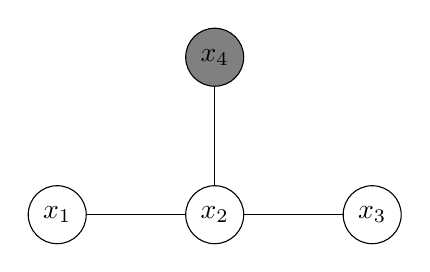
\begin{tikzpicture}
    \node[vertex] (1) at (-2,0) {$x_1$};
    \node[vertex] (2) at (0, 0) {$x_2$};
    \node[vertex] (3) at (2, 0) {$x_3$};
    \node[given] (4) at (0, 2) {$x_4$};
    \draw[edge] (1) --(2);
    \draw[edge] (2) --(3);
    \draw[edge] (2) --(4);
    \end{tikzpicture}
    \end{center}

$\psi_{12}(x_1, x_2) = \begin{bmatrix}
1.0 & 0.9\\
0.9 & 1.0\\
\end{bmatrix}, \psi_{23}(x_2, x_3) = \begin{bmatrix}
0.1 & 1.0\\
1.0 & 0.1\\
\end{bmatrix},\psi_{24}(x_2, x_4) = \begin{bmatrix}
1.0 & 0.1\\
0.1 & 1.0\\
\end{bmatrix},$ and suppose $x_4=0$
    
%\item TODO: Murphy exercise 20.3? 
    
\item Show BP on a HMM is exactly the forwards-backwards algorithm. 
\end{enumerate}





\end{document}